\documentclass[crop, tikz]{standalone}

\usepackage[utf8]{inputenc}
% 'crop' is the default for v1.0, before it was 'preview'
%\usetikzlibrary{...}% tikz package already loaded by 'tikz' option

\usetikzlibrary{arrows}
\usetikzlibrary{decorations.markings}
\usetikzlibrary{patterns}
\usetikzlibrary{calc}

%hexagon drawing variables
\def\ly{0.866025} %sin(pi/3) = sqrt(3)/2
\def\lx{0.5} %cos(pi/3) = 0.5
\def\hexSize{5} %size of the hexagon that'll be the extent of the fibre cross section
\def\coreSize{0.2} %size of hollow cores
\def\coreSep{0.5} %separation between core CENTRES HORIZONTALLY
\def\coreSepHeight{0.4464} %separation between core CENTRES VERTICALLY

\newcommand{\hexagon}[4]{
\begin{scope}[shift={#2}]
	\draw[#3, fill=#4] (-#1*\lx, #1*\ly) -- (#1*\lx, #1*\ly) -- (#1,0) -- (#1*\lx, -#1*\ly) -- (-#1*\lx, -#1*\ly) -- (-#1,0) -- cycle;
\end{scope}
} %\hexagon{centre-to-corner-length}{shift (x,y)}{line spec}{fill colour} [none is allowed for fillcolour]

\begin{document}
\newcommand{\grad}{\nabla}

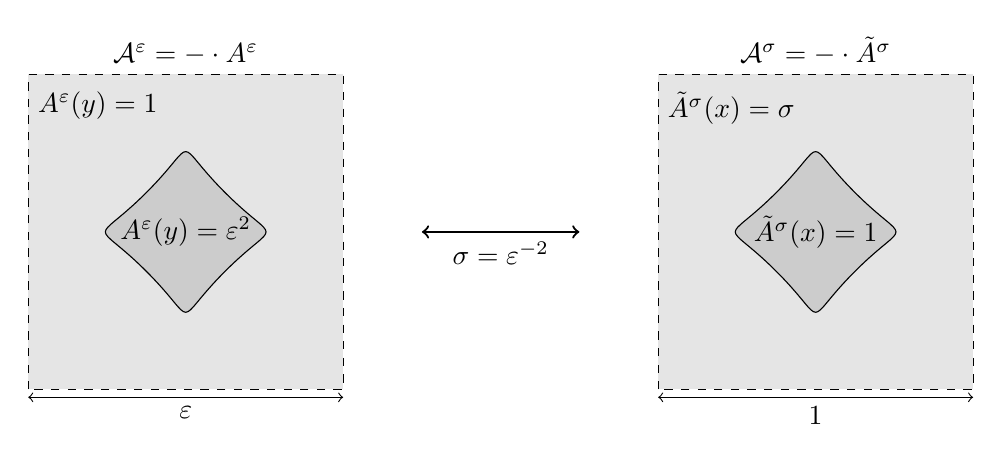
\begin{tikzpicture}[]

	\def\inc{black!20!white}
	\def\bulk{black!10!white}

	% Hempel-Lienau setup
	\begin{scope}[shift={(8,0)}]
		\filldraw[fill=\bulk, draw=black, dashed] (0,0) rectangle (4,4);
		\filldraw[fill=\inc, draw=black] plot [smooth cycle, tension=2.5] coordinates {(1.5,1.5) (2.5,1.5) (2.5,2.5) (1.5,2.5)};
		\draw[<->] (0,-0.1) -- (4,-0.1); 
		\node[anchor=north] at (2,-0.1) {$1$};
		\node[anchor=north west] at (0,3.9) {$\tilde{A}^{\sigma}(x)=\sigma$};
		\node[anchor=center] at (2,2) {$\tilde{A}^{\sigma}(x)=1$};
		\node[anchor=south] at (2,4) {$\mathcal{A}^{\sigma}=-\grad\cdot \tilde{A}^{\sigma}\grad $};
	\end{scope}

	% Zhikov double porosity model setup
	\begin{scope}[shift={(0,0)}]
		\filldraw[fill=\bulk, draw=black, dashed] (0,0) rectangle (4,4);
		\filldraw[fill=\inc, draw=black] plot [smooth cycle, tension=2.5] coordinates {(1.5,1.5) (2.5,1.5) (2.5,2.5) (1.5,2.5)};
		\draw[<->] (0,-0.1) -- (4,-0.1); 
		\node[anchor=north] at (2,-0.1) {$\varepsilon$};
		\node[anchor=north west] at (0,3.9) {$A^{\varepsilon}(y)=1$};
		\node[anchor=center] at (2,2) {$A^{\varepsilon}(y)=\varepsilon^2$};
		\node[anchor=south] at (2,4) {$\mathcal{A}^{\varepsilon}=-\grad\cdot A^{\varepsilon}\grad $};
	\end{scope}

	% link H-L to Zhikov
	\begin{scope}[shift={(6,2)}, scale=1.0]
		\draw[<->, thick] (-1,0) -- (1,0);
		\node[anchor=north] at (0,0) {$\sigma=\varepsilon^{-2}$};
	\end{scope}

\end{tikzpicture}

\end{document}